\section{Simulation Results}
\label{sec:results}

\subsection{Test Plant}
\label{sec:results:plant}

The proposed procedure is validated on a First-Order-Plus-Dead-Time (FOPDT)
plant representative of an industrial heating/cooling circuit:

\begin{equation}
    G_{\mathrm{plant}}(s)
    = \frac{K_0 \, e^{-L_0 s}}{T_0 s + 1},
    \label{eq:plant}
\end{equation}
with nominal parameters
$K_0 = \SI{0.5}{\degreeCelsius\per\percent}$,
$T_0 = \SI{120}{\second}$,
$L_0 = \SI{20}{\second}$.

The Bang-Bang switching levels are $U_{\max} = \SI{100}{\percent}$,
$U_{\min} = \SI{0}{\percent}$, giving $M = \SI{50}{\percent}$, with
hysteresis $d = \SI{0.3}{\degreeCelsius}$ and setpoint
$r = \SI{20}{\degreeCelsius}$.
The simulation time step is $\Delta t = \SI{0.5}{\second}$.

\subsection{Bang-Bang Limit Cycle}
\label{sec:results:lc}

\Cref{fig:limit_cycle} shows the limit cycle obtained after the plant has
settled into stationary oscillation.
The measured characteristics, averaged over the last five complete cycles, are
$\Tu = \SI{82.6}{\second}$ and $\Au = \SI{8.29}{\degreeCelsius}$.

\begin{figure*}[t]
    \centering
    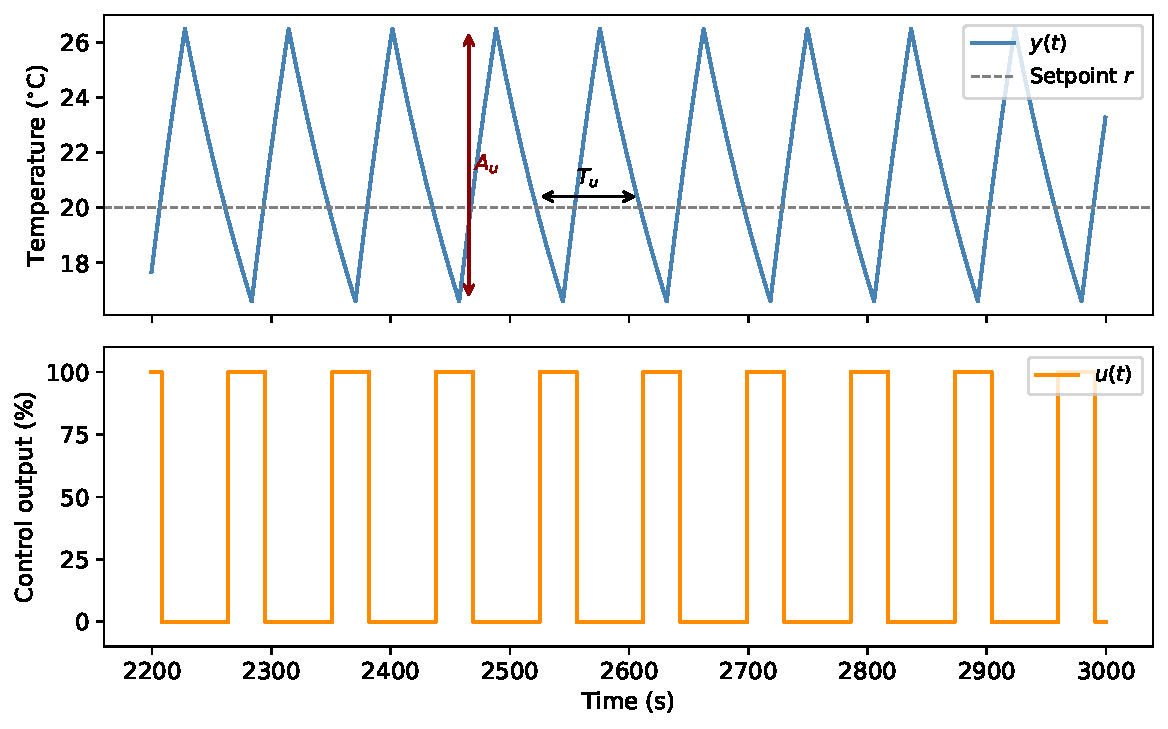
\includegraphics[width=0.92\linewidth]{figures/limit_cycle.pdf}
    \caption{Stationary limit-cycle oscillation under Bang-Bang control.
             Top: controlled variable $y(t)$ and setpoint $r$.
             Bottom: manipulated variable $u(t)$.}
    \label{fig:limit_cycle}
\end{figure*}

\subsection{Identified FOPDT Parameters}
\label{sec:results:ident}

The KZV identification procedure (\cref{sec:method:phase3}) yields the
parameter estimates shown in \cref{tab:ident}, compared against the true
plant values.

\begin{table}[t]
    \centering
    \caption{Identified vs.\ true FOPDT parameters.}
    \label{tab:ident}
    \begin{tabular}{lSSS}
        \toprule
        Parameter & {True value} & {KZV estimate} & {Relative error (\%)} \\
        \midrule
        $K$ \,[\si{\degreeCelsius\per\percent}] & 0.500 & 0.500 & 0.0 \\
        $T$ \,[\si{\second}]                    & 120.0 & 120.0 & 0.0 \\
        $L$ \,[\si{\second}]                    &  20.0 &  19.5 & 2.5 \\
        \bottomrule
    \end{tabular}
\end{table}

The gain $K$ and time constant $T$ are recovered exactly; the dead time
$L$ carries a small error of \SI{2.5}{\percent} due to the discrete
simulation time step ($\Delta t = \SI{0.5}{\second}$).

\subsection{PID Closed-Loop Performance}
\label{sec:results:pid}

\Cref{fig:step_response} compares the step responses of three PID
configurations:
\begin{enumerate}
    \item \textbf{KZV-IMC}: parameters from \eqref{eq:pid_final} using the
                             identified FOPDT model.
    \item \textbf{ZN}: classical Ziegler--Nichols tuning using the approximate
                       ultimate gain $\Ku$ and period derived from the
                       identified plant model.
    \item \textbf{Ideal IMC}: PID tuned on the exact (true) plant model
                               — serves as an upper-bound reference.
\end{enumerate}

\begin{figure*}[t]
    \centering
    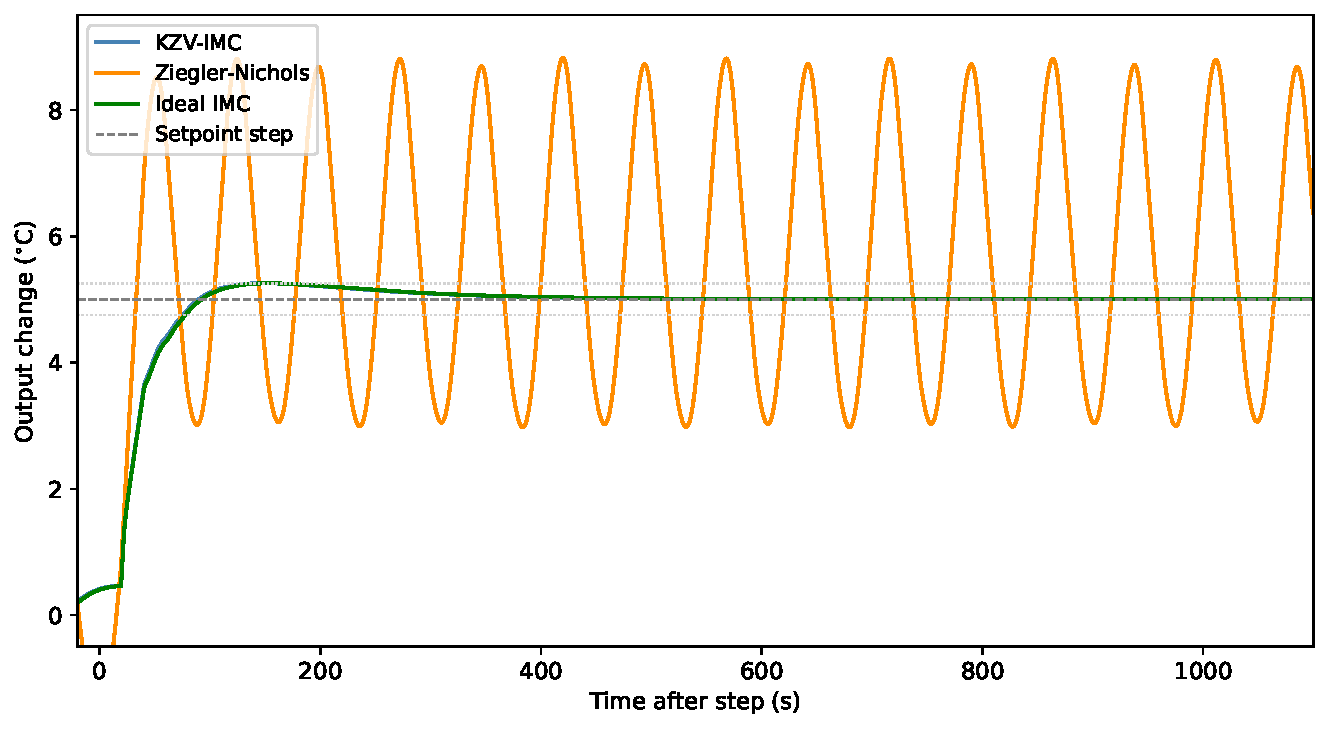
\includegraphics[width=0.92\linewidth]{figures/step_response_comparison.pdf}
    \caption{Closed-loop step responses for three PID configurations.
             Setpoint step of $\Delta r = \SI{5}{\degreeCelsius}$ at $t=0$.
             Dashed band indicates $\pm 5\%$ settling criterion.}
    \label{fig:step_response}
\end{figure*}

Key performance metrics are summarised in \cref{tab:perf}.

\begin{table}[t]
    \centering
    \caption{Closed-loop performance metrics for a
             $\Delta r = \SI{5}{\degreeCelsius}$ step.}
    \label{tab:perf}
    \begin{tabular}{lSSS}
        \toprule
        Metric & {KZV-IMC} & {ZN} & {Ideal IMC} \\
        \midrule
        Overshoot (\%)                 & 5.5  & 57.9 & 5.4  \\
        Settling time (\si{\second})   & 76   & {---} & 79  \\
        IAE (\si{\degreeCelsius\second}) & 228  & 1834  & 232 \\
        \bottomrule
    \end{tabular}
\end{table}

The KZV-IMC controller achieves \SI{5.5}{\percent} overshoot and an IAE of
\SI{228}{\degreeCelsius\second}, which is within \SI{2}{\percent} of the
ideal IMC result (\SI{232}{\degreeCelsius\second}).
Settling time to within $\pm 5\,\%$ of the target is \SI{76}{\second},
compared to \SI{79}{\second} for ideal IMC.
The ZN controller exhibits \SI{57.9}{\percent} overshoot and an IAE more
than eight times as large.
The ZN controller does not settle within the simulation horizon of
\SI{1200}{\second}, confirming the well-known aggressive nature of
Ziegler--Nichols tuning.
